\documentclass[tikz]{standalone}

\usepackage{amsmath}
\usepackage{tikz}
\usetikzlibrary{matrix}
\usetikzlibrary{backgrounds}

\begin{document}

\begin{tikzpicture}


    \node at (0, 0) (pic) {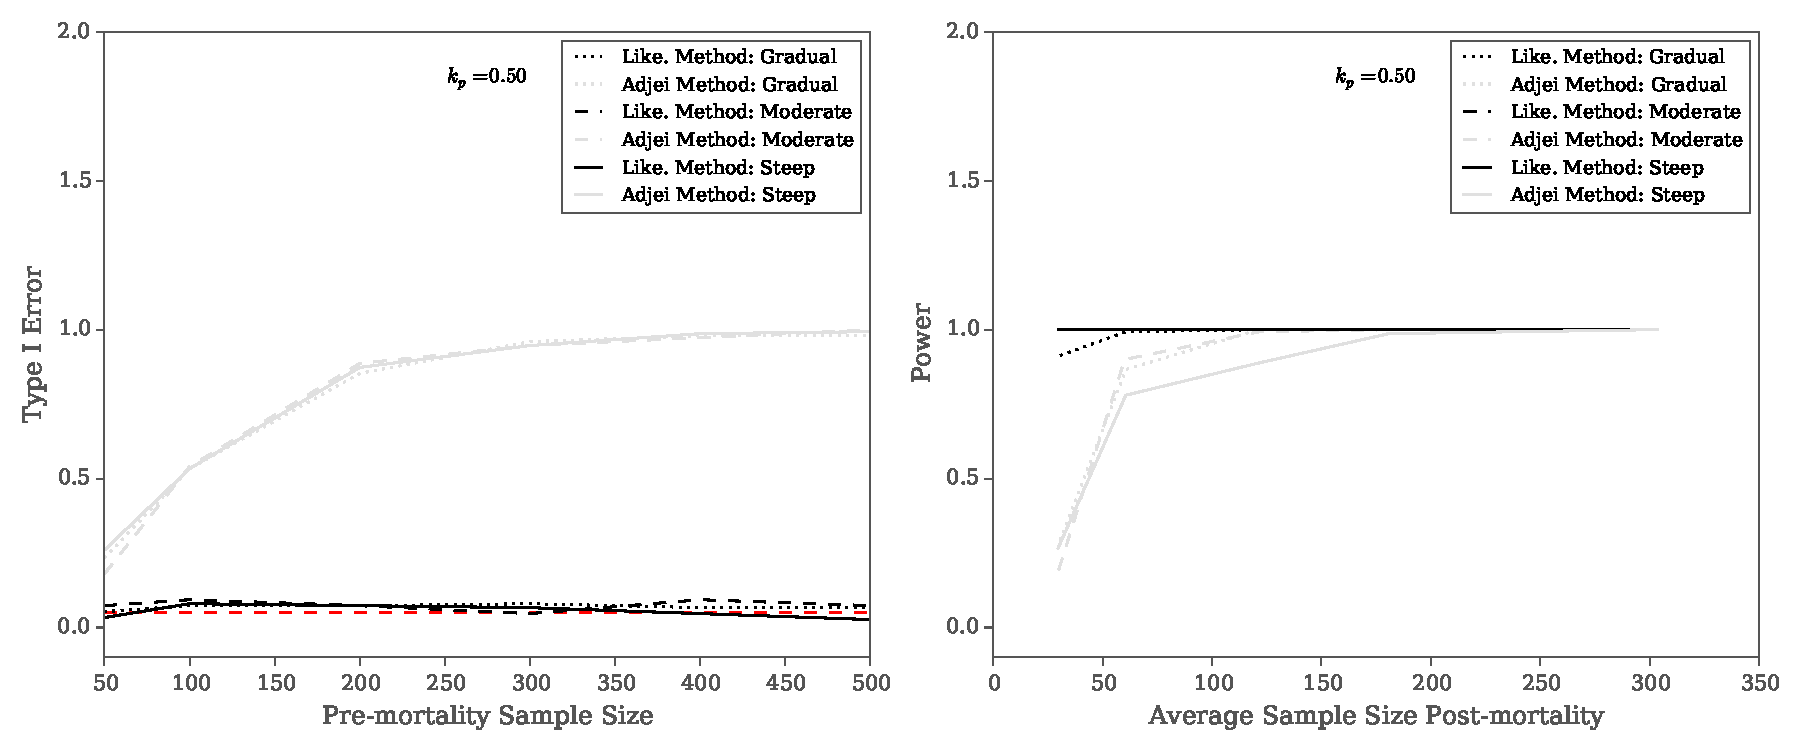
\includegraphics[width=\textwidth]{/Users/mqwilber/Repos/parasite_mortality/results/figure1_partII_for_manuscript50}};

    \node[above=0.1cm] at (pic.north) (concept) {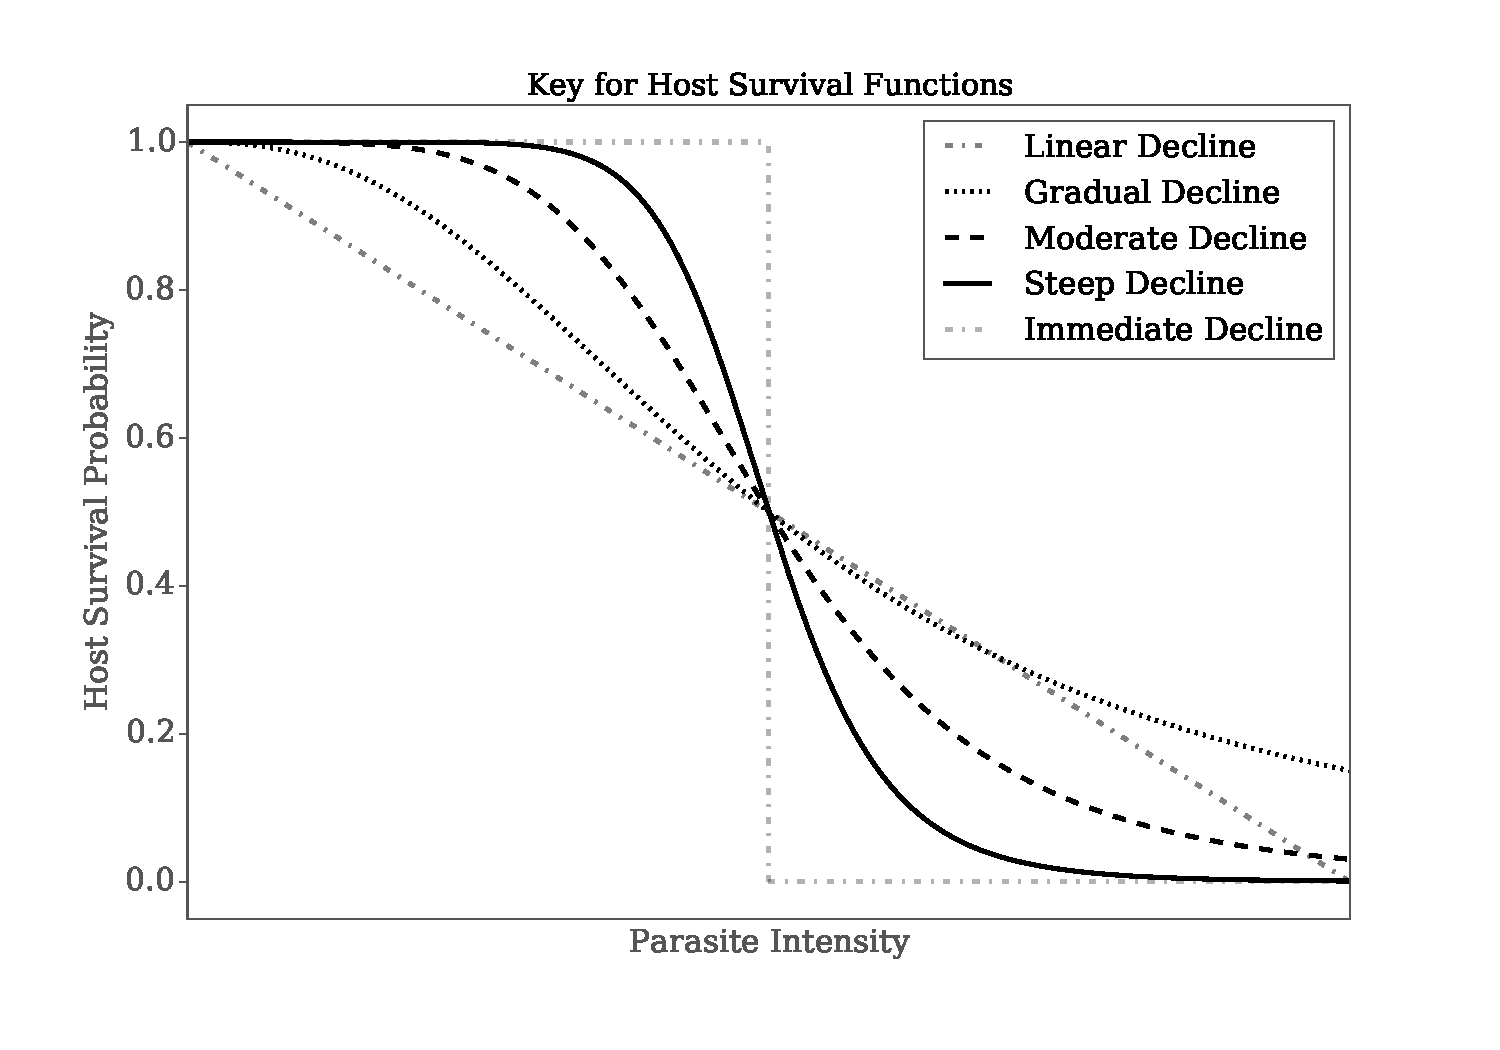
\includegraphics[width=0.6\textwidth]{/Users/mqwilber/Repos/parasite_mortality/results/figure1_partI_for_manuscript}};

    \draw[->] (0, 4.2)--(-1.5, 3.2);
    \draw[->] (0, 4.2)--(1.5, 3.2);

    \node at (-2.5, 3.8) {A.};
    \node at (-5, 2.2) {B.};
    \node at (1, 2.2) {C.};

\end{tikzpicture}

\end{document}